\section{Equations}
Typeset the following. Some hints:
\begin{itemize}
    \item Make sure to decide the right environment (\texttt{align, align*, equation}, etc) and where you want to horizontally align.
    \item To get squiggly brackets \verb|{}|, use: \verb|\{ text here \}|.
    \item For normal text in math mode, use \verb|\text{text here}|.
\end{itemize}

\begin{enumerate}
    \item Use \verb|\,| to space \verb|dx| properly.
        \begin{equation*}
            f(x) = \int_{0}^{2\pi} \sin(2x) \,dx
        \end{equation*}
    \item Use \verb|\dot{}| and \verb|\implies|.
        \begin{align*}
            \sum \dot{m} = 0 \implies \rho \sum u_i A_i = 0
        \end{align*}
    \item Use \verb|\partial|.
        \begin{equation*}
            \frac{\partial}{\partial y} \left[
                e^{-\alpha xy} \left( \frac{\alpha - 2}{x} \right)
            \right]
            =
            \frac{\partial}{\partial x} \left[
                -\frac{1}{\alpha y} \left(
                    e^{- \alpha xy} - 1
                \right)
            \right]
        \end{equation*}
    \item Use \verb|\therefore|.
        \begin{align*}
            & i(t) = i_C(t) + i_R(t) \\
            & d(t)I = C \frac{d}{dt}v_{out}(t) + \frac{v_{out}(t)}{R} \qquad \{\text{Laplace transform}\} \\
            & D(s)I = \left( Cs + \frac{1}{R} \right)V_{out}(s) \\
            & \therefore \frac{V_{out}(s)}{D(s)} = \frac{RI}{RCs+1}
        \end{align*}
    \item Use \verb|\vec{}| and the \verb|bmatrix| environment
    \begin{equation*}
        \vec{\varepsilon} =
            \begin{bmatrix}
                \Delta L_x/L_x \\ \Delta L_y/L_y \\ \Delta L_z/L_z
            \end{bmatrix}
        =
            \begin{bmatrix}
                0.975-1 \\ 0.975-1 \\ 1.05-1
            \end{bmatrix}
        =
            \begin{bmatrix}
                -0.025 \\ -0.025 \\ 0.05
            \end{bmatrix}
    \end{equation*}
\end{enumerate}

\section{Graphs}
Graph the following using \texttt{tikz}/\texttt{pgfplots}:
\begin{enumerate}
\item \( f(x)=x^2 \), domain = -2:2
\item \( f(x) = \sin(2x)  \), domain = 0:2$\pi$, axis lines = left

\begin{figure}[h]\centering
\begin{tikzpicture}
    \begin{axis}[
        xlabel = \(x \), ylabel = \(f(x)\), axis lines = left, domain=0:2*pi
    ]
        \addplot[samples=150] {sin(deg(2*x))};
    \end{axis}
\end{tikzpicture}
\end{figure}

\textbf{Hints:}
\begin{itemize}
    \item Make sure to convert \verb|2*x| to degrees using \verb|deg(2*x)|
    \item You may need to increase the number of \texttt{samples} in the plot. Use the option \texttt{samples=150}. 
\end{itemize}
\clearpage
\item Recreate the following logistic curve, including drawn comment.
\begin{figure}[h]
\centering
\begin{minipage}{0.35\textwidth} \centering
    Curve's function:
    \begin{equation*}
        f(x) = \frac{2}{1+e^{-2(x-0.5)}}    
    \end{equation*}
    \verb|= 2/(1+exp(-2*(x-0.5)))|
\end{minipage}
\begin{minipage}{0.60\textwidth}
    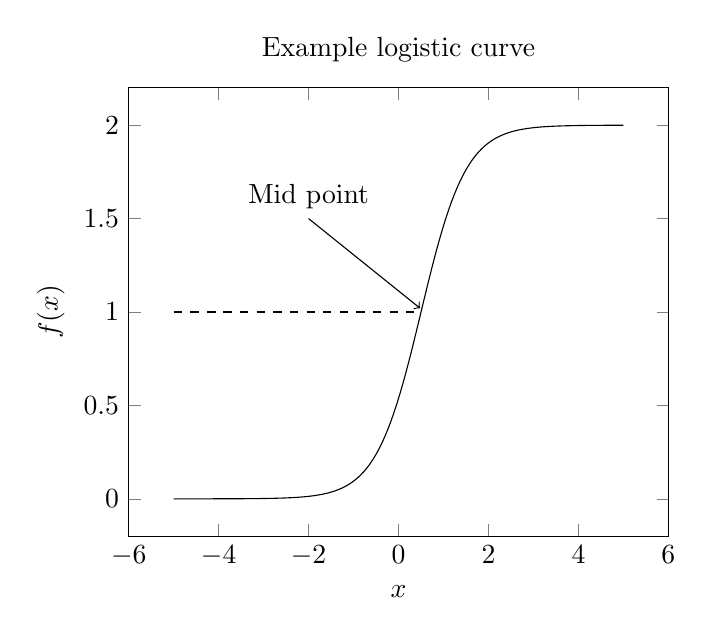
\begin{tikzpicture}
        \begin{axis}[
            xlabel = \(x \), ylabel = \(f(x)\), title=Example logistic curve,
        ]
            \addplot[samples=150] {2/(1+exp(-2*(x-0.5)))};
            \addplot[dashed, domain=-5:0.5] {1}; 
            \draw[->] (axis cs: -2,1.5) node[above] {Mid point} -- (axis cs: 0.48,1.02);
        \end{axis}
    \end{tikzpicture}
\end{minipage}
\end{figure}

\textbf{Hints:}
\begin{itemize}
    \item In order to draw inside an axis at coordinate \verb|(x,y)|, we use \verb|(axis cs: x,y)|.
    \item In the example, the arrow is from \texttt{(-2,1.5)} to \texttt{(0.48,1.02)}
\end{itemize}
\item Recreate the following graph. The function is \( f(x) = \frac{1}{2} (1-e^{-2x})\). 
\begin{figure}[h]\centering
    \begin{tikzpicture}
    \begin{axis}[
        xlabel=t, ylabel=y(t), title=System response,
        axis lines = middle,
        legend pos = outer north east,
        align=center, clip=false, scale=1.3
    ]
    \addplot[blue,samples=100, domain=0:10] {1/2*(1- exp(-2*x))} ;
    \addlegendentry{$v_{out}(t)$};
    \addplot[red,thick, domain=0:10] {1};
    \addlegendentry{$v_{desired}(t)$}
    \addplot[domain=-2:0,red,thick] {0};
    \draw[->] (axis cs: 8,0.53) -- (axis cs: 8,0.98) node[midway, right](){Steady-state \\ error};
    %%Dashed lines
    \draw[dashed] (axis cs: 0.5,0) -- (axis cs: 0.5,0.32) ;
    \addplot[dashed, domain=0:0.5] {0.32};
    \addplot[dashed, domain=0:2] {0.5};
    \end{axis}
    \end{tikzpicture}
    \caption{System response given a step input}
    \end{figure}
\end{enumerate}